\chapter{Einleitung}\label{ch:intro}

In den letzten Monaten und Jahren bringen Neuronale Netze viele \textit{State-of-the-Art} Ergebnisse in beinahe allen möglichen Disziplinen des Maschinellen Lernens hervor. Eine der Disziplinen ist das Natural Language Processing, kurz \textit{NLP}. Unter diesem Begriff verbergen sich noch viele weitere weitverbreitete Disziplinen, unter Anderem sentiment analysis, machine translation, voice recognition und auch text generation. Da die Textgeneration auch \textit{Sprachmodellierung} genannt, ein Kernelement einiger NLP-Disziplinen ist, gibt es viele Vorgängerversionen. Vor einigen Jahren wurden hauptsächlich die beiden Ansätze des Regelbasierten-Sytems und des Templatebasierten-Systems (Figure \ref{rules_based}) verwendet, wohingegen \textit{State-of-the-Art} die Neuronalen Ende-zu-Ende Systemen sind.  Diese neuen Systeme bieten wesentlich mehr Flexibilität und skalieren weit bessere Ergebnisse mit wegen benötigten Daten, da die Komplexität und somit die benötigte Rechenleistung drastisch gestiegen ist. Aus dieser Tatsache heraus ergibt allerdings ein Komplexitätsproblem, da es sehr schwer wird die Entscheidungen des Neuronalen Netzes nachzuvollziehen. Das Neuronale Netz ist weitestgehend immer noch eine \textit{Black Box}, obwohl es erstaunlich gute Ergebnisse liefert, vor allem im NLP. Nichtsdestotrotz sind Neuronale Netz Modelle um Text zu verarbeiten schlecht zu verstehen, deswegen müssen heutzutage immer noch Kompromisse zwischen den Regelbasierten System geschlossen werden und Hybride Systeme verwendet werden. 

\begin{figure}
  \begin{center}
  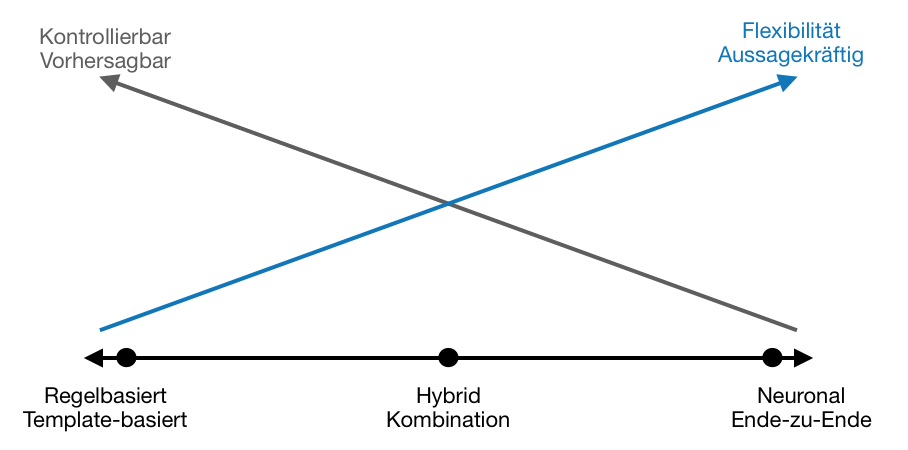
\includegraphics[width=3.5in]{photos/regel_basiert}\\
  \caption{Regelbasiertes- vs. Neuronales Text generations System}\label{rules_based}
  \end{center}
\end{figure}

Die natürliche Text Generation, auch \textit{NTG} genannt, hat wiederum viele nützliche und interessante Einsatzgebiete. Darunter zählen  
\begin{itemize}
\item Spracherfassung und Umwandlung in Text
\item Konversationssysteme z.B. Chatbots
\item Textzusammenfassung
\end{itemize} 

Um Sprachmodelle zu trainieren muss ihnen die Wahrscheinlich von auftretenden Wörtern in Abhängigkeit der vorangegangen Wörter beigebracht werden. Es gibt mehrere Ansätze um dieses Ziel zu erreichen. Sprachmodelle können auf Ebene der Wörter, ganzer Sätze oder sogar ganze Paragraphen trainiert werden. Die Granularität in welcher das Training stattfindet wird als \textit{n-grams} bezeichnet, wovon  \textit{n} die Anzahl der vorangegangen Wörter repräsentiert.

\section{Fallbeispiel eines aktuellen NLP-Systems}

\subsection{Fallbeispiel}

Image-to-Text | Captionbot Microsoft

\subsection{Nützliche Einsatzgebiete von NLP-Systemen}

IoT, Grammerly

\subsection{Nützliche Einsatzgebiete von NTG-Systemen}